\documentclass[../src/handouts/main.tex]{subfiles}
% note that the CWD (.) above is the output directory of pdflatex
% (<repo-root-dir>/build)

% path that contains required images
\graphicspath{ {../src/handouts/figures/} }

% This document depends on the other sections, which provide the
% following references (in the order of references in this section):
%   enum:con-tree-state
%   prop:con-connected-vertex
% As a result, compiling only this document gives undefined references.

% prevent \recall theorems outside this section
% if this section is compiled solely
\def\sectionprefix{tree}%

\begin{document}

\section{Trees and Distance}

This section is the chapter 2 in the textbook "Introduction to Graph Theory".

\supp{Tree and its techniques (breadth first search, depth first search) are common in programming contest, computer aided design (CAD), software verification, logic analysis, etc. As a result, this section is important in this course.}

\begin{definition}{}{tree-tree}
  A graph with no cycle is \textbf{acyclic}.

  A \textbf{forest} is an acyclic graph.

  A \textbf{tree} is a connected acyclic graph.

  A \textbf{leaf} (pendant vertex, terminal) is a vertex of degree 1.

  A \textbf{spanning subgraph} of $G$ is a subgraph with vertex set $V(G)$.

  A \textbf{spanning tree} is a spanning subgraph that is a tree.
\end{definition}

\begin{figure}[htbp]
  % TODO: TikZ version
  \centering
  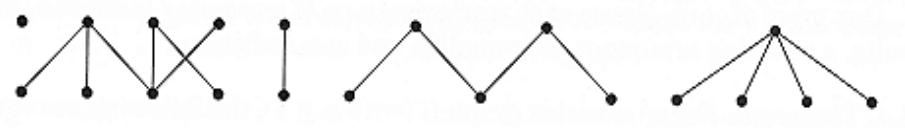
\includegraphics[width=.6\textwidth]{tree-tree-introduction}
  \caption{Examples of forests and trees.}
\end{figure}

\begin{lemma}{}{tree-deleting-leaf}
  (2.1.3. Lemma in text)
  Every tree with at least two vertices has at least two leaves.
  Deleting a leaf from an $n$-vertex tree produces a tree with $n-1$ vertices.
\end{lemma}

A graph with only two vertices and an edge is also a tree by definition, so such a graph is covered by \cref{lem:tree-deleting-leaf}.

\textbf{Proof} of \cref{lem:tree-deleting-leaf}:
\begin{enumerate*}
  \item \supp{In this proof, it is better to have at least 3 nodes in a tree. However, in the textbook it used a tree with 2 vertices as an example.}
  \item In a tree (connected acyclic graph) with at least 3 nodes, an endpoint of a maximal nontrivial path has no neighbor other than its neighbor on the path. Hence the endpoints of a such a path are leaves.
  \item Let $v$ be a leave of a tree $G$ of three nodes, and let $G' = G - v$.
  \item A vertex of degree 1 (vertex $v$) belongs to no path connecting two other vertices. Therefore, for $u, w \in V\left( G' \right)$, every $u,w$-path in $G$ is also in $G'$. Hence $G'$ is connected. Since deleting a vertex cannot create a cycle, $G'$ is also acyclic. Thus $G'$ is a tree with $n - 1$ vertices.
\end{enumerate*}

\begin{figure}[htbp]
  % TODO: TikZ version
  \centering
  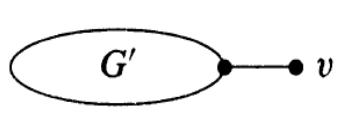
\includegraphics[width=.3\textwidth]{tree-deleting-leaf}
  \caption{An illustration of deleting a leaf $v$ from $G$ to form $G'$.}
  \label{fig:tree-deleting-leaf}
\end{figure}

\begin{theorem}{}{tree-tree-stat}
  (2.1.4. Theorem in text; introduced in \cpageref{enum:con-tree-state} previously)

  For an $n$-vertex graph $G$ (with $n \geq 1$ ), the following statements are equivalent (and characterize the trees with $n$ vertices).
  \begin{enumerate*}
    \item $G$ is connected and has no cycles.
    \item $G$ is connected and has $n - 1$ edges.
    \item $G$ has $n - 1$ edges and no cycles.
    \item For $u, v \in V(G)$, $G$ has exactly one $u,v$-path.
  \end{enumerate*}
\end{theorem}

Traditionally, to prove \cref{thm:tree-tree-stat}, we need to prove these 4 statements pairwisely (6 iff. pairs). Nonetheless, in this proof, we prove any two of the statements \{ connected, acyclic, $n - 1$ edges\} for a graph imply the other one, and prove the statement 4 is equivalent to any of the three statements, saying statement 1 (connected and acyclic), with 4 iff. pairs in total instead of 6.

Note that your assumption must be correct before any proof. For example, these 4 statements must be correct before proofs. Under wrong assumptions, you have only wrong results.

\textbf{Proof} of statement 1 (connected, acyclic) implying statements 2 and 3 ($n - 1$ edges) in \cref{thm:tree-tree-stat}:

\begin{enumerate*}
  \vspace{-.25em} % magic number to make these enumerated list look alike
  \item We use induction on $n$, which is the number of vertices in the graph $G$.
  \item For $n = 1$, an acyclic 1-vertex graph has no edge.
  \item For $n > 1$:
    \vspace{.5em}
    \begin{enumerate*}
      \item We suppose that the implication holds for graphs with fewer than $n$ vertices.
      \item Given an acyclic connected graph $G$, \cref{lem:tree-deleting-leaf} provides a leaf $v$ and states that $G' = G - v$ also is acyclic and connected (see figure above).
      \item Applying the induction hypothesis to $G'$ yields $e \left( G' \right) = n - 2$. Since only one edge is incident to $v$, we have $e(G) = e \left( G' \right) + 1 = n - 1$.
    \end{enumerate*}
    \vspace{.25em} % more space after enumerate*
\end{enumerate*}
\vspace{.5em} % more space after enumerate*

\textbf{Proof} of statement 2 (connected, $n - 1$ edges) implying statements 1 and 3 (acyclic) in \cref{thm:tree-tree-stat}:
\begin{enumerate*}
  \item We use proof by contradiction.
  \item Suppose the graph $G$ has a cycle.
  \item Delete edges from cycles of $G$ one by one to form $G'$ until the resulting graph $G^{\prime}$ is acyclic. \supp{We cannot delete edges that are not parts of some cycles, or we will make the graph disconnected (no path from a component to the other one).}
  \item Recall \cref{prop:con-connected-vertex}: The minimum number of edges in a connected graph with $n$ vertices is $n - 1$.
  \item To have $G'$ connected, $e\left( G' \right) = n - 1$.
  \item Since we are given $e(G) = n - 1$, no edges were deleted. Thus $G' = G$, and $G$ is acyclic.
\end{enumerate*}
\vspace{.5em} % more space after enumerate*

\textbf{Proof} of statement 3 ($n - 1$ edges, acyclic) implying statements 1 and 2 (connected) in \cref{thm:tree-tree-stat}:
\begin{enumerate*}
  \item We use proof by contradiction with some calculation.
  \item Let $G_1,\, \ldots,\, G_k$ be the components of $G$. If $k \geq 2$, then $G$ is disconnected.
  \item Since every vertex appears in a single component, $\sum_i n \left( G_i \right) = n$. Since $G$ has no cycles, $e \left( G_i \right) = n \left( G_i \right) - 1$ for each $i$.
  \item Summing over $i$ yields $e(G) = \sum _i \left( n \left( G_i \right) - 1 \right) = n - k$.
  \item We are given $e(G) = n - 1$, so $k = 1$, and $G$ is connected.
\end{enumerate*}
\vspace{.5em} % more space after enumerate*

\textbf{Proof} of statement 1 (connected, acyclic) implying statement 4 (unique $u,v$-path) in \cref{thm:tree-tree-stat}:
\begin{enumerate*}
  \item We use proof by contradiction.
  \item Since the graph $G$ is connected, each pair of vertices is connected by a path. \supp{We cannot say that these is no path to violate the assumption of a conencted graph.}
  \item If some pair ov vertices $u,\, v$ is connected by \textbf{more than one path}, a cycle is formed by any two of the paths as illustrated in \cref{fig:tree-tree-stat}. It contradicts to the assumption of an acyclic graph.
  \item As a result, there is only a single path between any two vertices in $G$.
\end{enumerate*}
\vspace{.5em} % more space after enumerate*

\clearpage % magic escape to prevent paragraph overlapping with the footer
\textbf{Proof} of statement 4 (unique $u,v$-path) implying statement 1 (connected, acyclic):
\begin{enumerate*}
  \item We use direct method and proof by contradiction.
  \item If there is a $u,v$-path for every $u,\, v \in V(G)$, then $G$ is connected.
  \item If $G$ has a cycle $C$, then $G$ has two $u,v$-paths for $u,\, v \in V(C)$. It contradicts to the assumption that there is only a single path between $u$ and $v$.
  \item Hence, $G$ is acyclic (this also forbids loops).
\end{enumerate*}
\vspace{.5em} % more space after enumerate*

\begin{figure}[htbp]
  % TODO: TikZ version
  \centering
  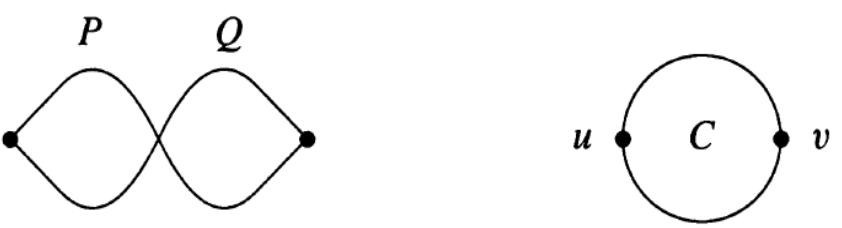
\includegraphics[width=.5\textwidth]{tree-tree-stat}
  \caption{A graph to illustrate the proof of equivalence between statements 1 and 4 in \cref{thm:tree-tree-stat}.}
  \label{fig:tree-tree-stat}
\end{figure}

\end{document}